% !TEX root = ../main.tex

\chapter{Research paper experiment reproduction}
\label{ch:paper_reproduction}
\setlength{\marginparwidth}{3cm}\leavevmode \marginnote{\textbf{Jobin}}This chapter is based on the article "Computer-Aided Diagnosis of Prostate Cancer Using a Deep Convolutional Neural Network from Multiparametric MRI" from Song et al.~\cite{07}, shortly presented in Chapter \ref{ch:literature_review}. It aims at reproducing the experiment of the paper in order to acquire the medical, theoretical and technical background before proposing a transfer learning method as a way to improve the classification using other body parts (see Chapter \ref{ch:transfer_learning}).

Song et al.~\cite{07} proposed a deep convolutional neural network (DCNN) method to detect prostate cancer based on the SPIE-AAPM-NCI PROSTATEx Challenge dataset. This dataset is one of the biggest datasets available for prostate cancer classification. The two different output classes of the latter are benign lesion (class 0) and malignant lesion (class 1). The dataset contains a total of 204 patients for the training (labels are known) and 208 patients for the challenge (labels are unknown). This paper explains all the steps to follow with the goal of building a deep learning model for prostate cancer detection. Moreover, it also provides results (AUC) about the algorithm performance on a test set they built themselves (which is not the same as the challenge test set). In fact, they split the PROSTATEx training set into a training set, a validation set and the mentioned test set. These results can be used as a benchmark to compare with the results of the reproduction of the experiment. However, the article gives no information about the results their model achieved on the official PROSTATEx challenge test set (208 patients without labels). Therefore, the reproduction of the experiment will fill that gap by taking part in the actual challenge.

This chapter is built in a top-down fashion. First, an overview of the entire process is established in order to understand the purpose of the experiment as a whole. Then, each theoretical notion is described in detail. This includes the structure of the dataset, the steps involved in its processing, and the techniques used as a verification of the proper functioning of the algorithm. Then, the training phase is dealt with in depth and all hyperparameters, options and implementation choices are described to ensure the reproductibility of the experiment. This part is followed by the presentation of the raw results the model achieved on the test set (the one built for the experiment), which is itself followed by their analysis in the "Discussion" section. Finally, the last section is devoted to the so-called SPIE-AAPM-NCI Prostate MR Classification Challenge. It presents the results that the model achieved on the challenge test set using the whole training set for the training. The latter section is not part of the original paper.
%and represents the contribution of this work to it.

\section{Process overview}
\setlength{\marginparwidth}{3cm}\leavevmode \marginnote{\textbf{Jobin}}Schematically speaking, the entire experiment process can be represented as shown on Figure \ref{fig:paper_reproduction_process}. The first part of the experiment is about the reproduction of the paper experiment, whereas the second one is devoted to the participation in the SPIE-AAPM-NCI PROSTATEx challenge since the authors of the article did not take part in it.

\subsubsection{Experiment reproduction}
The first part of the experiment makes use of the PROSTATEx training set. This dataset is only composed of samples whose clinical significance is provided (labeled data). The first step of the reproduction is the data processing. In fact, many processing steps are involved to transform the original DICOM files into NumPy arrays which can be fed to the neural network. Data processing includes lesion cropping, normalization, MRI images stacking, data augmentation, etc. (see Section \ref{sec:prostatex_data_processing} for further details).\\
Once the processing part is completed, the labeled data are split into a training set, a validation set and a test set using respectively 80\%, 10\% and 10\% of the available data for each subset. The training set samples are then fed to the neural network in batches. 
%, which updates its weight consequently. 
At the end of each epoch, the current model is tested on the validation set and the resulting metrics are plotted in Tensorboard (see Section \ref{paper_tensorboard}). The validation set is independent of the training set and has never been seen by the model, which gives an indication of how well the latter generalizes. Then, if the current model reaches a higher AUC and a higher accuracy than the previous best model, it becomes the new best model and it is saved. Furthermore, if the validation AUC decreases for a defined number of epochs, the learning rate is reduced to prevent overfitting and avoid a progressive decrease in validation performance. This technique contributes to maintaining a good generalization level and optimizes the training with respect to the AUC.\\
As soon as the training phase reaches the defined number of epochs, the model is tested on the test set with the authors' method called "enhanced prediction" to compute the AUC. The latter method consists in predicting an output for each augmented test image before averaging the predictions for each lesion of each patient.

\subsubsection{PROSTATEx challenge}
The second part of the experiment relies on the results of the first one. Indeed, the same data processing pipeline is applied and the hyperparameters used to train the neural network are the same. The difference lies in the fact that the entire dataset (i.e. the entire PROSTATEx training set) is used as training set instead of splitting the data into a training, validation and test sets. In this way, the model sees more training examples, which maximizes the performance of the model on the challenge test set by increasing its generalization ability. During the training phase, the model is saved at the end of each epoch. Once the training is over, multiple models are chosen around the epoch that produced the best result on the validation set during the first part of the experiment. These models are then evaluated on the challenge test set by submitting their predictions for each lesion to the Grand Challenge organization. The model with the best result on the challenge is considered as the most efficient one.

\clearpage

\begin{figure}[!t]
\centering
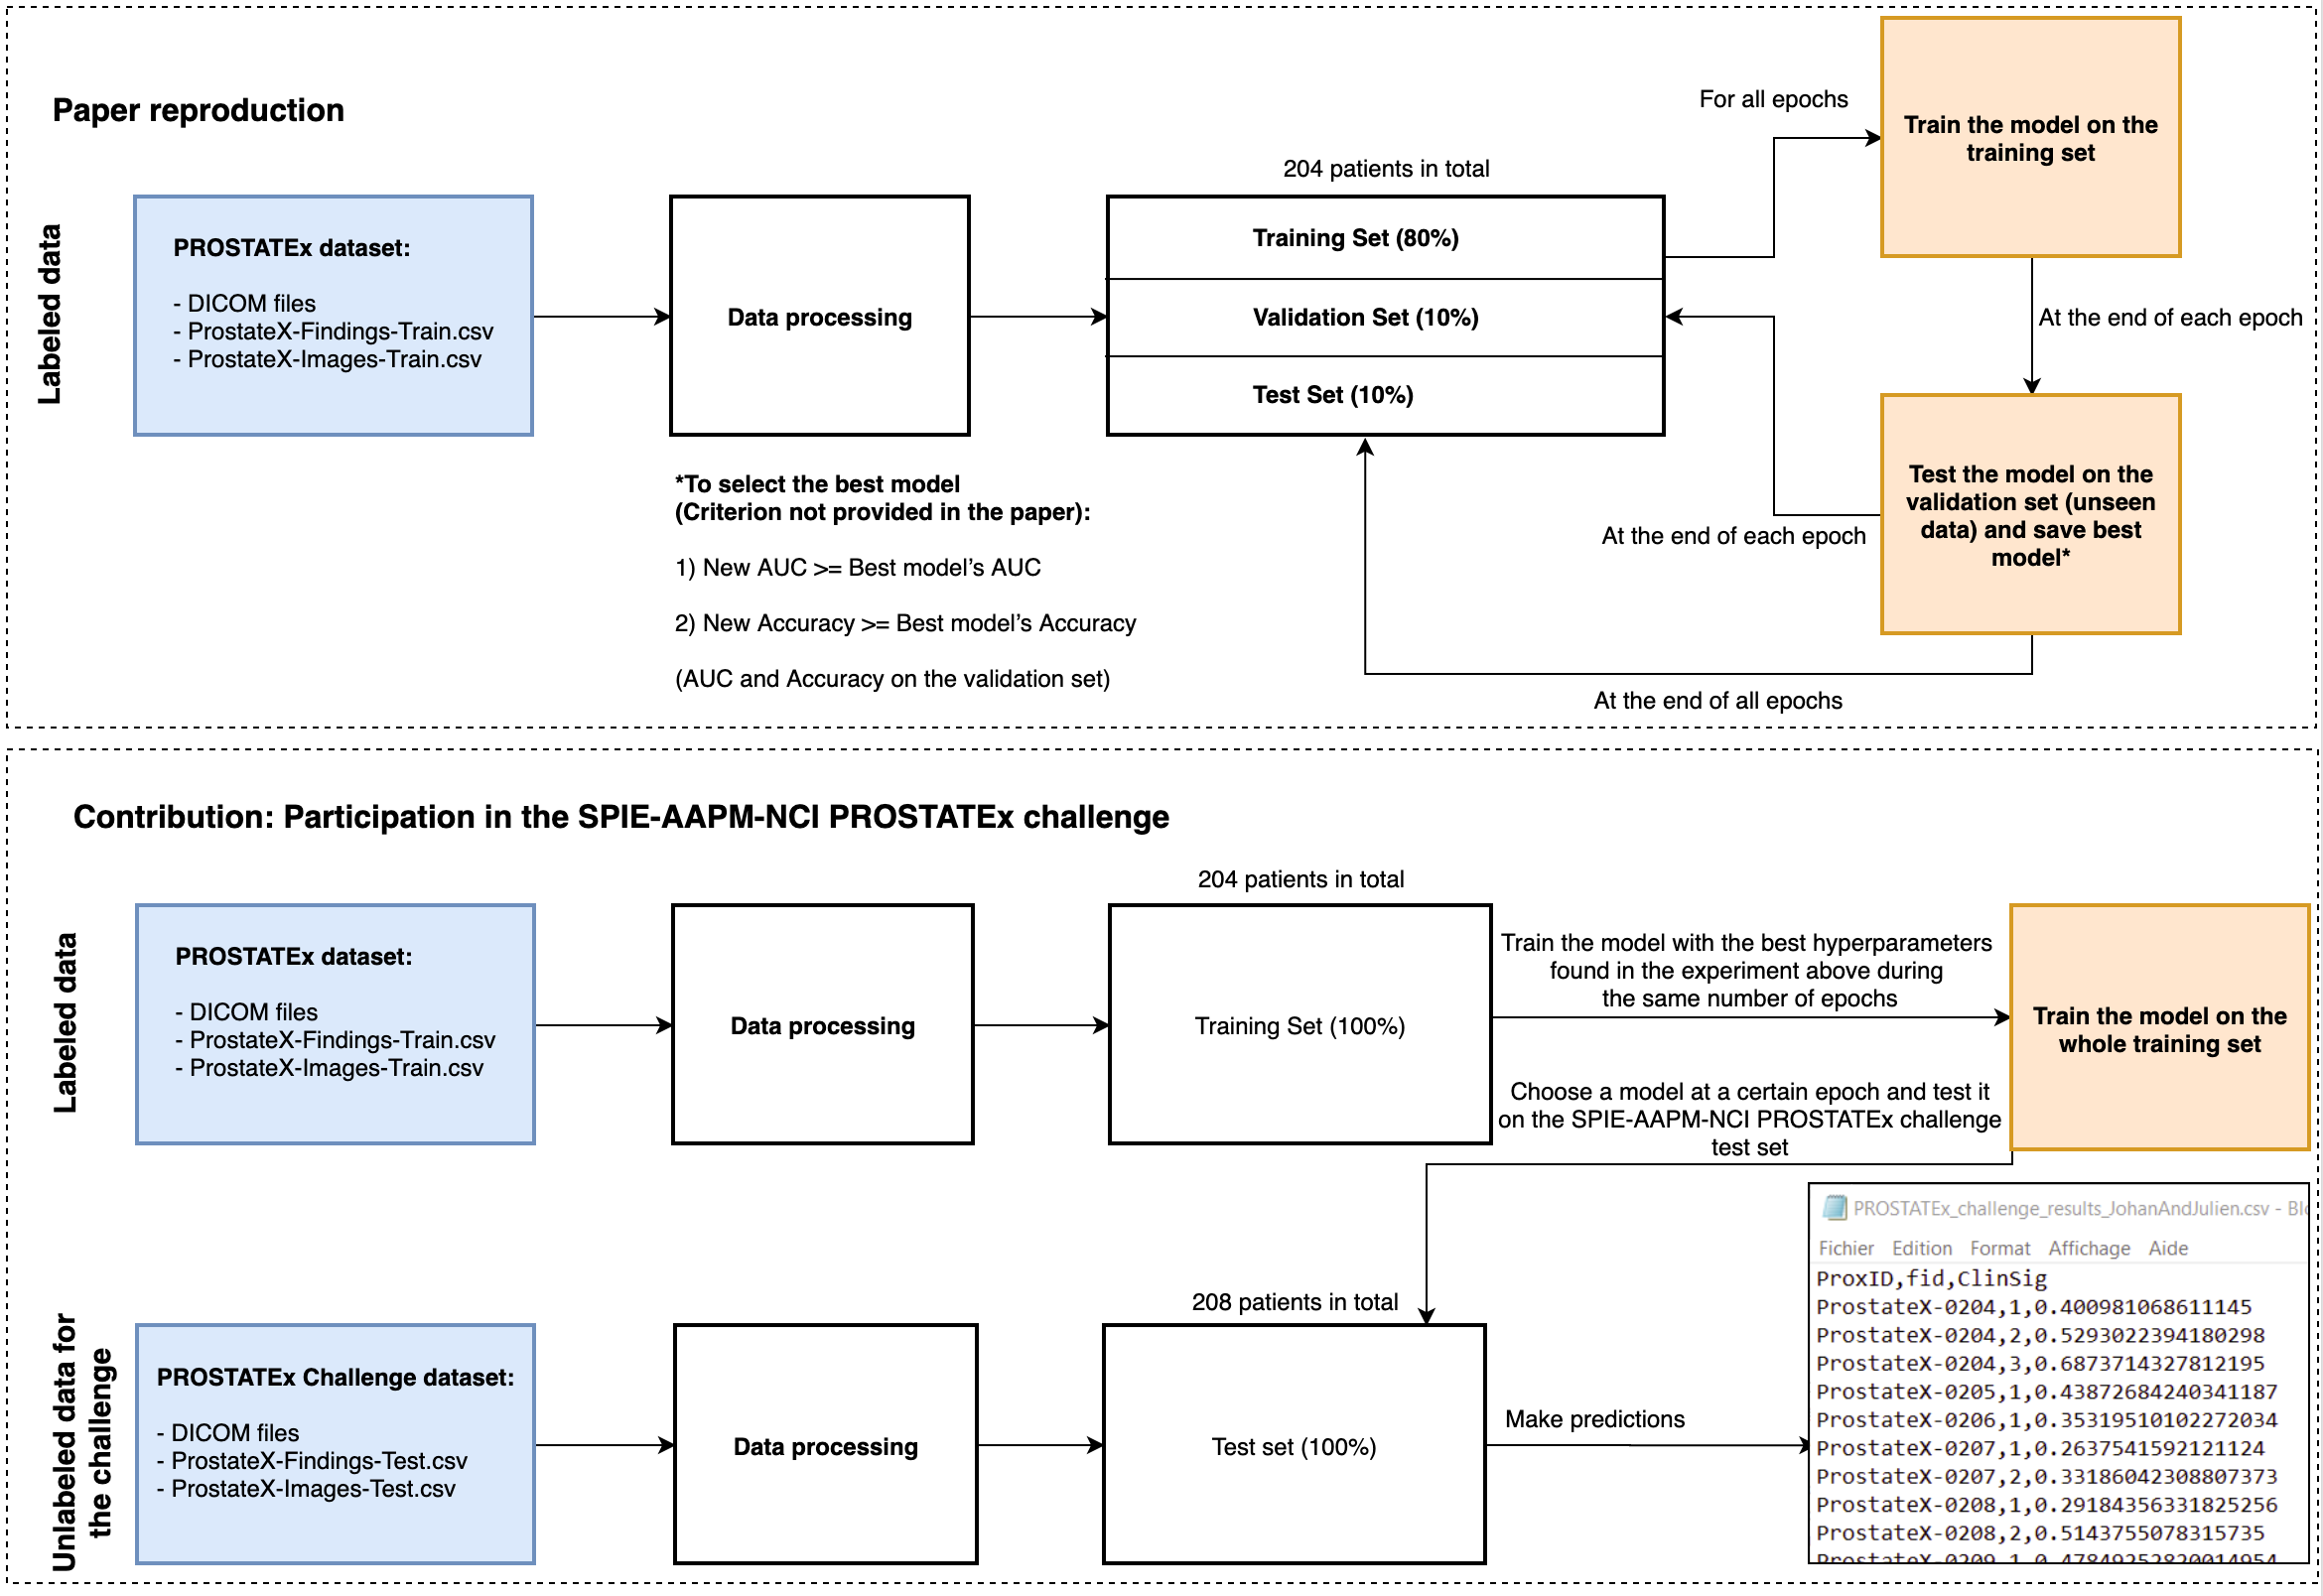
\includegraphics[width=1\textwidth, keepaspectratio=true]{./figures/paper_reproduction_process.png}
\caption{Overview of the whole experiment process}
\label{fig:paper_reproduction_process}
\end{figure}

\section{Reproducing the paper experiment}

\subsection{PROSTATEx: Data processing}
\label{sec:prostatex_data_processing}
\setlength{\marginparwidth}{3cm}\leavevmode \marginnote{\textbf{Cl{\'e}ment}}This section describes the processing operations performed on the raw data until it passes through the neural network. All steps mentioned below are also valid for the second part of the experiment about the challenge (Section \ref{sec:classification_challenge}).


\subsubsection{Dataset description}
\label{sec:prostatex_dataset_description}
\setlength{\marginparwidth}{3cm}\leavevmode \marginnote{\textbf{Cl{\'e}ment}}The SPIE-AAPM-NCI PROSTATEx Challenge dataset is publicly available on the Cancer Imaging Archive website~\cite{33, 34, 35}. This dataset is composed of multiparametric MRIs for a total of 204 training patients and 208 challenge patients. Images were taken under the sagittal, transverse and coronal planes. These MRIs are multiparametric because the same exam was performed using different radiological settings called "sequences". Each sequence allows to see human tissue in a different way on the resulting images. The sequences available within the scope of PROSTATEx are T2 weighted images (T2W), Diffusion weighted images (DWI), Apparent diffusion coefficient (ADC), Dynamic contrast enhanced (DCE), PD (Proton Density) and K-trans. The PROSTATEx dataset comes with two CSV files for the training set:
\begin{itemize}
\item The first one, \textit{ProstateX-Findings-Train.csv}, lists all findings with their clinical significance. Multiple findings can belong to the same patient (ProxID).

\item The second one, \textit{ProstateX-Images-Train.csv}, gives information about where to find the right DICOM file for each patient and each finding. Important labels are "ProxID" (patient ID), "fid" (finding ID $\in [1,\infty]$), "ClinSig" (clinical significance, TRUE or FALSE), "DCMSerNumber" (digit before the dash in the folder name containing DICOM files), "ijk" (position of the lesion: slice number $k$ at coordinates $(i,j)$, $i,j,k \in [0,\infty]$) and "VoxelSpacing" (3-dimensional vector representing the correspondance between a pixel and the space it occupies in the real world). Both CSV files are complementary to each other. 
\end{itemize}

\noindent Regarding the challenge patients, two analog CSV files are provided: \textit{ProstateX-Findings-Test.csv} and \textit{ProstateX-Images-Train.csv}. The only difference is the absence of clinical significance. Finally, images are in the DICOM file format (see \mbox{Section \ref{sec:DICOM}}). 


\subsubsection{Methodology}
\setlength{\marginparwidth}{3cm}\leavevmode \marginnote{\textbf{Cl{\'e}ment}}The methodology described in this section is the closest replication possible of the authors' data processing methodology. Most of it were reproductible in a similar way, apart from the manual lesion contouring which was performed by a qualified radiologist in the authors' case. Furthermore, the authors did not mention any participation in the official PROSTATEx challenge.

In order to get an unbiased evaluation of the performance of our model, these images were also processed as explained below in order to take part in the challenge, but were not augmented. Nevertheless, the authors created their own test set by splitting the PROSTATEx training images into a training set ($80\%$), a validation set ($10\%$) and a test set ($10\%$). They mentioned that the test set was augmented $11$ times but gave no information about the training and validation sets. Since the training set is imbalanced (3 false for 1 true), the true class was augmented more times than the false class (which was augmented $60$x) in order to create balanced training and validation sets. 


\subsubsection{From DICOM to NumPy arrays}
\label{sec:DICOMtoNumPy}
\setlength{\marginparwidth}{3cm}\leavevmode \marginnote{\textbf{Cl{\'e}ment}}Before anything else, T2W, DWI and ADC grayscale images were used, which means that DCE, PD and Ktrans images were left aside. Furthermore, DWI images regroup various parameters which create different subcategories. One of them is the so-called "b-value" which is "a factor that reflects the strength and timing of the gradients used to generate diffusion-weighted images. The higher the b-value, the stronger the diffusion effects"~\cite{49}. The authors tested three different b-value configurations. This led to the conclusion that using DWI images with the highest b-value increased the performance of the model. For that matter, DWI images with the highest b-value only were used in this work. Moreover, only images showing the prostate under the transverse plane were used. The reason for this is that the tumors are much more visible under this perspective. 

The first step consisted in converting PROSTATEx's DICOM files to NumPy arrays. Algorithm \ref{alg:PROSTATEx_preprocessing} describes the steps involved in this process. The right slices were found thanks to the two CSV files. Important information such as the patient ID, the sequence, the lesion location and the voxel spacing was included in the file output names, which allows to use these files independently for the next steps (i.e. without relying on the CSV files) that consist in stacking and augmenting the images. Furthermore, this information is also extremely useful for the visualization and verification scripts in order to provide concrete details regarding the displayed images.

\begin{algorithm}
    \caption{PROSTATEx preprocessing}
    \label{alg:PROSTATEx_preprocessing}
    \begin{algorithmic}[1] % The number tells where the line numbering should start
        \Procedure{main}{$dataset\_folder, findings\_CSV, slices\_CSV, output\_folder$}
        		\State Create output directories: $"output\_folder/True", "output\_folder/False"$\\
        		\State $findings \gets read\_CSV(findings\_CSV)$ \Comment{ProstateX-Findings-Train.csv}
        		\State $slices \gets read\_CSV(slices\_CSV)$ \Comment{ProstateX-Images-Train.csv}
			\State $meta \gets merge(findings, slices)$\Comment{Both CSV files are complementary to each other.}\\
            \For{$row$ in $meta$}
            		\State $patient\_id \gets row["ProxID"]$
            		\State $finding\_id \gets row["fid"]$
            		\State $mri\_type\_number \gets row["DCMSerNumber"]$
            		\State $clinical\_significance \gets row["ClinSig"]$
            		\State $img\_i, img\_j, img\_k \gets row["ijk"]$
            		\State $slice\_number \gets img\_k + 1$ \Comment{CSV indexing in $[0,\infty]$, DICOM in $[1,\infty]$}\\
                \For{$visit\ in\ patient\_id$'s folder}
                		\For{$mri\_type$ in $visit$}
                			\If {$mri\_type$ starts with "$mri\_type\_number$-"}
                				\For{$dicom\_file$ in $mri\_type$}
                					\If {$slice\_number == dicom\_file.InstanceNumber$}
                						\State{$slice \gets normalize\_dicom(dicom\_file)$} \Comment{see Section \ref{sec:dicom_data_manipulation}}
                						\State{Save $slice$ in $"output\_folder/clinical\_significance"$}
                					\EndIf
                				\EndFor
                			\EndIf
            			\EndFor
            		\EndFor
            \EndFor
        \EndProcedure
    \end{algorithmic}
\end{algorithm} 

\newpage

\subsubsection{From NumPy arrays to augmented stacked images}
\label{sec:numpyToAugmentedStacked}
\setlength{\marginparwidth}{3cm}\leavevmode \marginnote{\textbf{Jobin \& Cl{\'e}ment}}This step can be split into two substeps: aligning and stacking images before augmenting them and splitting them across a training set, a validation set and a test set.

Once full images were converted to NumPy arrays, the images related to a specific lesion of a specific patient needed to be aligned and resampled to the same resolution. In fact, T2-weighted images have a much higher resolution than the DWI and ADC images (in this dataset at least). Without this operation, a single pixel on a DWI image would have covered a lot more tissue than a pixel of the corresponding T2 image. To perform the alignment, the lesion was localized on the three sequences than to the CSV file. Then, the goal was to crop a large patch which contained the same amount of tissue on the three images. This patch had to be centered on the lesion to ease the augmentation process. So, a fixed patch size was defined for the T2 image since its resolution was the highest. Then, using the voxel spacing information, the patch size required to cover the same amount of tissue was computed for the two other sequences (DWI, ADC). Finally, the three images were cropped, resized to the same resolution and stacked. Stacking images consists in putting each single image (grayscale) into a single array, as three different channels. At this point, the pixel $i,j$ of the three channels represents the exact same tissue, which means that the lesion is at the same position and is covered by the same number of pixels on each channel. This approach increases the probability of detecting a cancer by ensuring a good visibilty for each lesion, as the latter is not necessarily as visible on the three images.

An important part of this process is the normalization. In fact, images were normalized before beeing stacked, based on a Z-score, i.e. 
\begin{equation}
\label{eq:normalization}
	Pixel_{{i,j}_{normalized}} = \frac{Pixel_{i,j} - \mu}{\sigma}
\end{equation}
\noindent where $Pixel_{i,j} \in [0,255]$ is a grayscale pixel value, $\mu$ is the mean value of all images of the corresponding sequence for this patient and $\sigma$ the standard deviation of all images of the corresponding sequence for this patient. According to the authors, normalizing each sequence of each patient separately allows to keep slight contrast nuances which ultimately help the final diagnosis. In other words, all T2-weighted images belonging to a specific patient were concatenated into a single NumPy array. Then, the mean and standard deviation of the array were computed. These values served as $\mu$ and $\sigma$ to normalize the T2-images of this specific patient. The equivalent was applied to the patient's DWI and ADC images, and the same process was employed for all patients separately.
Then, the dataset was augmented in the same way as the authors. Concretely, images were rotated ($-20$ to $20^\circ$), flipped horizontally (probability of $0.5$) and shifted horizontally (value $\in [-1, 0, 1]$ pixel). These techniques alone allowed to create a large enough amount of data. Therefore, two other augmentation methods used by the authors (horizontal stretching by a \mbox{factor $\in [0.9,1.1]$} and vertical shifting) were not used.

On the other hand, authors did not mention how they managed class imbalance. It seems like the manual lesion contouring performed by the qualified radiologist led to a natural class balance. However, the unmodified dataset has a ratio of 3 negative images for 1 positive. To solve this problem, multiple approaches were implemented. The first one made use of undersampling which consists in taking N elements of each class, where N is the size of the class whose number of elements is the smallest. As the size of the dataset is relatively small, taking a subset of it was not a good idea and led to a clear lack of data. The second solution solved the problem by using different augmentation factors. In fact, one of the script options sets the augmentation factor for the class whose number of elements is the largest. Then, according to this factor, the algorithm computes the augmentation factor for the other class in order to balance the final datasets. For example, if the dataset follows the above-mentioned 3 negatives for 1 positive ratio, and if the script option augmentation factor is set to 50, each image belonging to the negative class is going to be augmented 50 times and each image belonging to the positive class 150 times. At the end, the resulting dataset is balanced and makes use of all images.

Finally, the data was split into three subsets (training ($80$\%), validation ($10$\%) and test ($10$\%)) and was exported as NumPy arrays. The percentages represent a percentage of patients. Figure \ref{fig:paper_reproduction_split} explains the entire splitting process and gives details about the patients that are in each set. In fact, each subset contains respectively 80\%, 10\% and 10\% of all patients belonging to the "true" and "false" class. At the beginning of the process, class "false" contains $\lfloor 0.8 * 164 \rfloor = 131$ training patients, $\lfloor 0.1 * 164 \rfloor = 16$ test patients and $164 - 131 - 16 = 17$ validation patients. On the other hand, class "true" contains $\lfloor 0.8 * 69 \rfloor = 55$ training patients, $\lfloor 0.1 * 69 \rfloor = 6$ test patients and $69 - 55 - 6 = 8$ validation patients. Then, during the stacking process, some patients were not used since the three sequences were not available for them. These patients were simply discarded. At the end, the "false" class contained 131 training patients, 17 validation patients and 15 test patients, whereas the "true" class contained 55 training patients, 8 validation patients and 4 test patients. This approach does not take the number of images into account (a patient may have multiple lesions for example) but guarantees that every lesion is exclusive to a specific subset. In other words, it is impossible to find a slighty different version of the same lesion (resulting from the data augmentation) in the training set and in the validation set for example. This would be problematic since the validation set, as well as the test set, need to contain unseen data to be able to evaluate the generalization ability of the model in an unbiased way. 

\begin{figure}[!h]
\centering
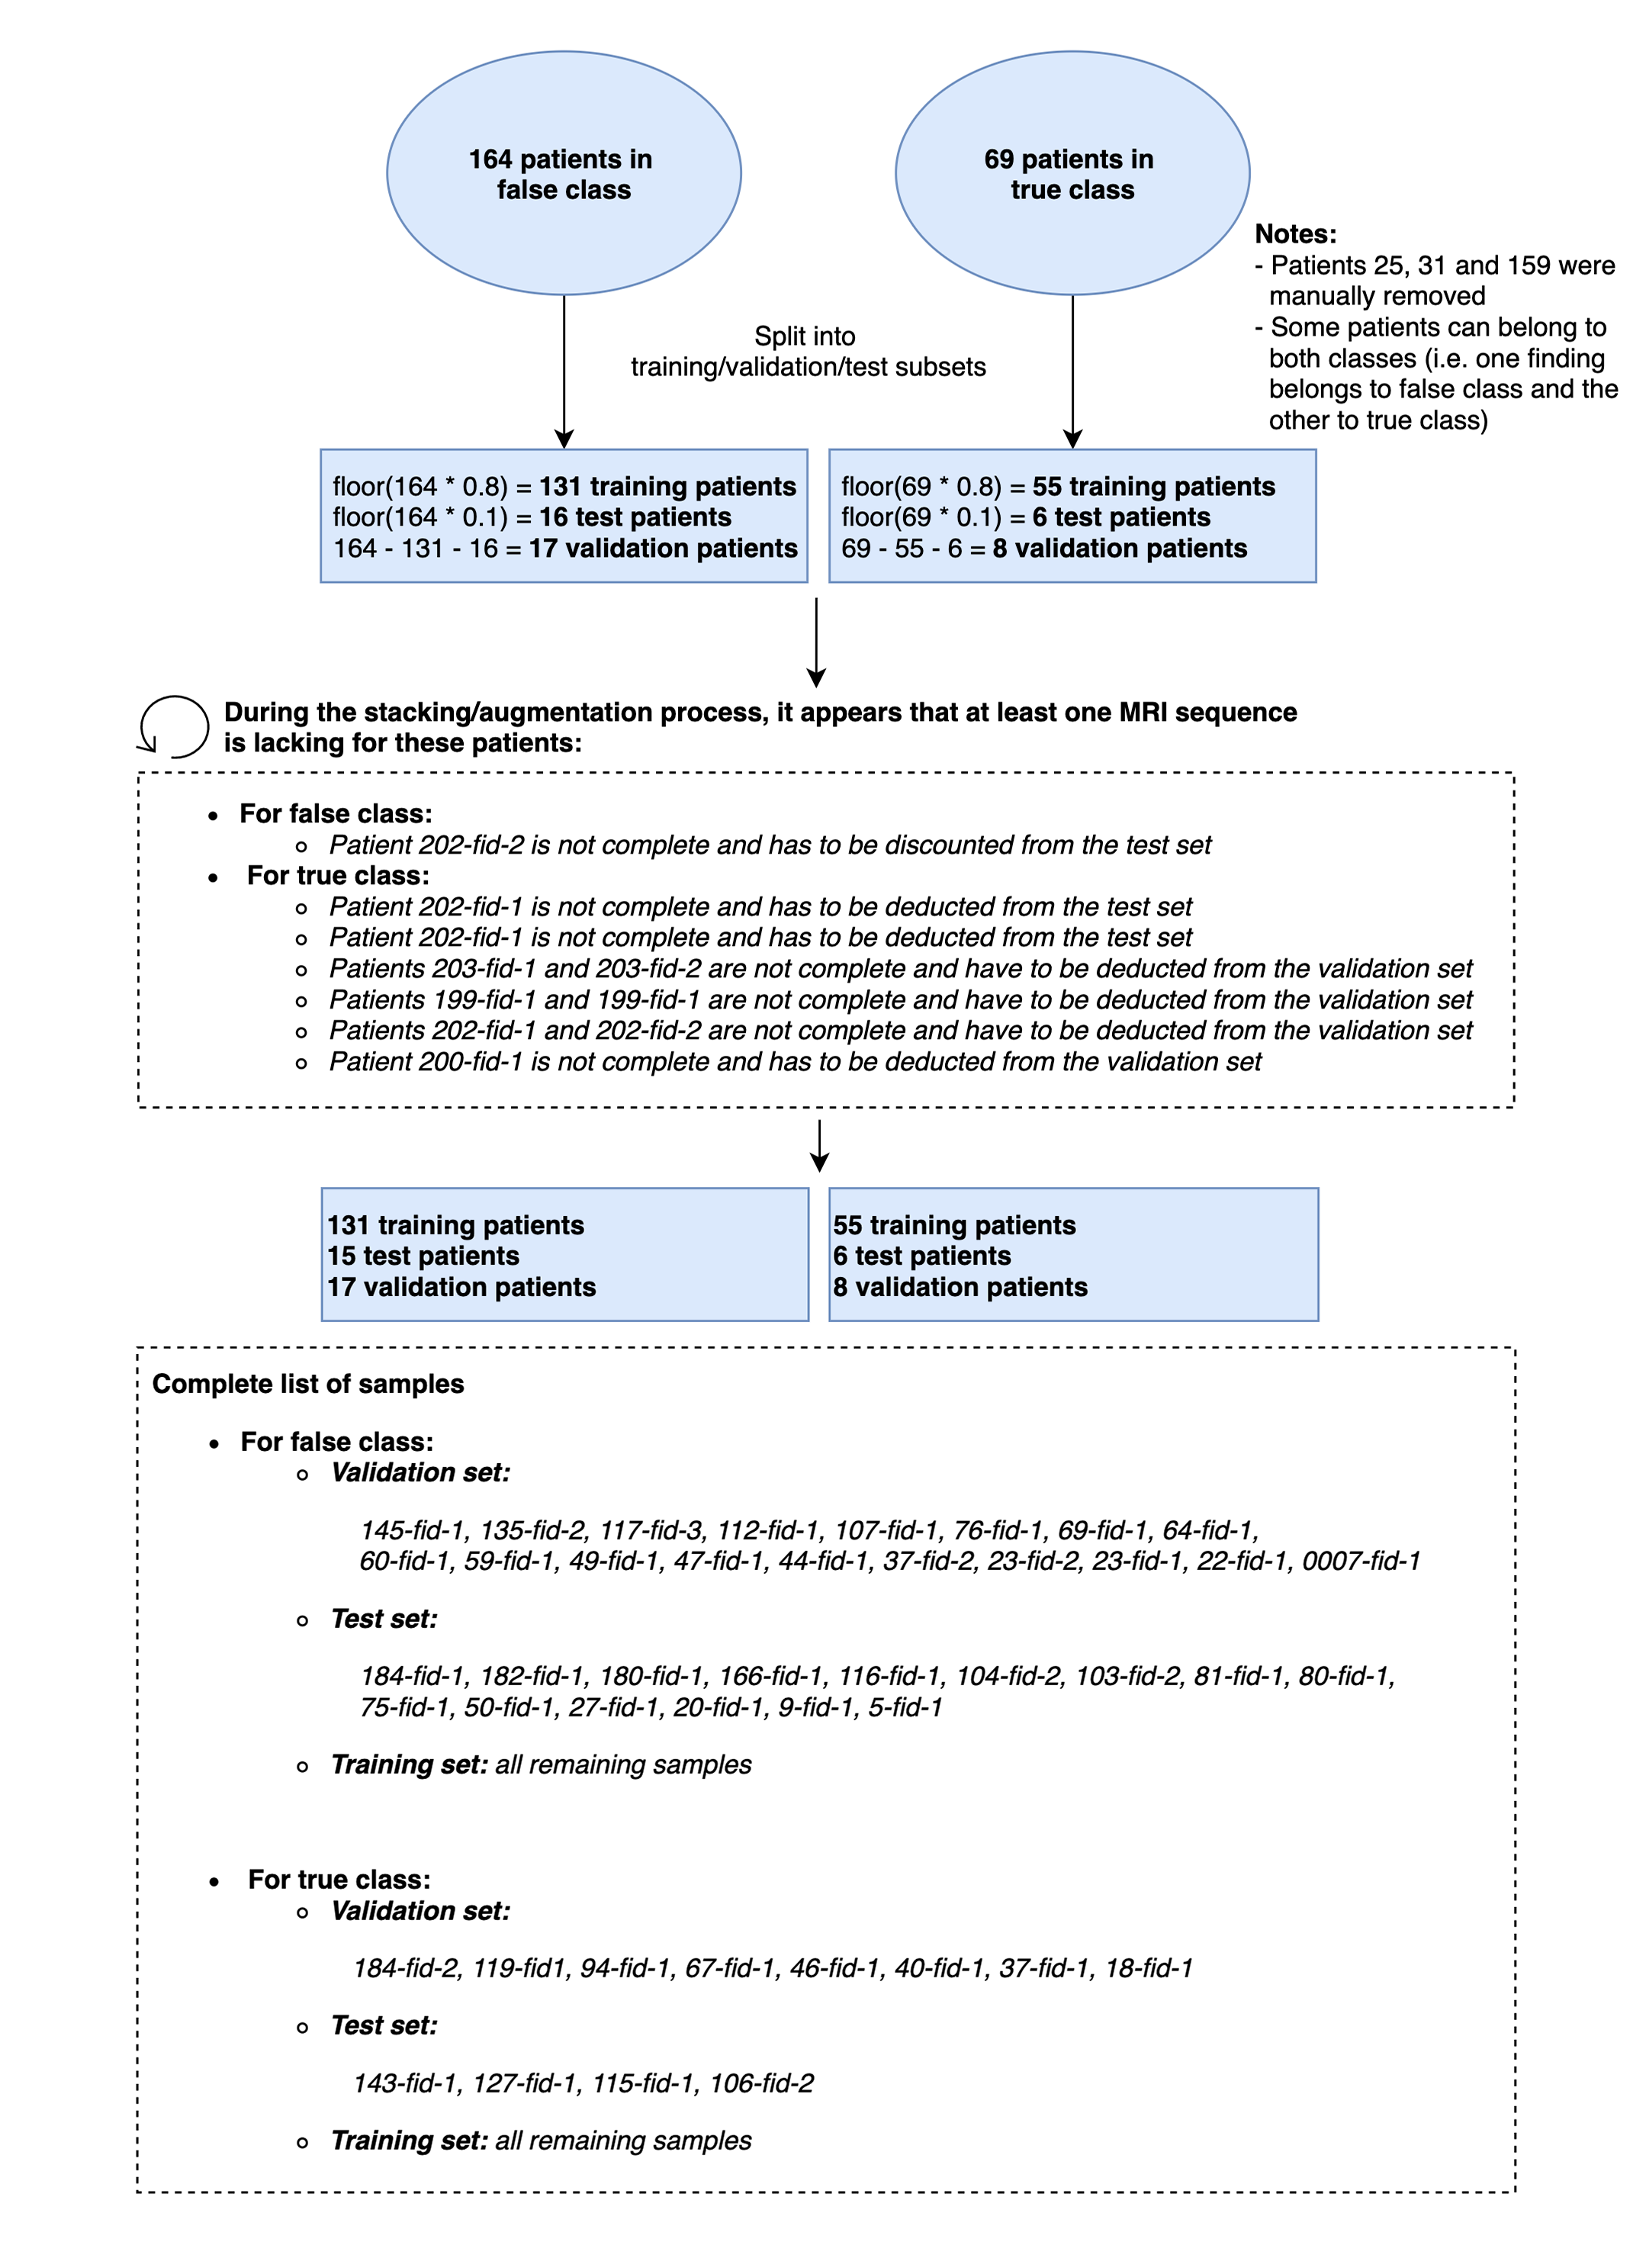
\includegraphics[width=1\textwidth, keepaspectratio=true]{./figures/paper_reproduction_split.png}
\caption{Patient splitting process}
\label{fig:paper_reproduction_split}
\end{figure}


\subsubsection{From NumPy arrays to augmented non-stacked images}
\setlength{\marginparwidth}{3cm}\leavevmode \marginnote{\textbf{Cl{\'e}ment}}Another way of processing and using the data was tested. Instead of stacking the images of various sequences coming from the same exam, each image was treated independently. In other words, each of them was resized as explained previously, then cropped, augmented and exported separately. At the end, each image was fed as separate input to the neural network.

This way of proceeding gave awful results. The main reason is that images from different sequences show the same tissue in an almost opposite way. The most striking difference to the human eye is the colors. Tumors are usually white on DWI images and black on ADC images. Moreover, they are not always as visible on the images of the various sequences. Therefore, finding similar features on all sequences is extremely difficult. Stacking the three sequences solves this problem. 
%In this case, the first 4225 input neurons (4225 input neurons for a $65$x$65$px image) are dedicated to T2 images, the next 4225 neurons to DWI images and the last 4225 neurons to ADC images. 


\subsection{Data processing verification}
\label{sec:dataProcessingVerification}
\subsubsection{Cropping verification using red dots}
\setlength{\marginparwidth}{3cm}\leavevmode \marginnote{\textbf{Cl{\'e}ment}}In order to check the correctness of the augmentation process, images with a red dot at the lesion coordinates were generated. First of all, a red dot was placed on the full image thanks to the "i,j,k" attribute of the CSV file. This full image was exported. Then, images were augmented in the exact same manner as described in Section \ref{sec:numpyToAugmentedStacked}. The expected result satisfies the following properties:
\begin{itemize}
	\item The red dot is localized in the center of the cropped and augmented image.
	\item The three cropped and augmented images within a stacked image contain the exact same tissue. 
	\item The three cropped and augmented images within a stacked image are not rotated/shifted/flipped differently. 
	\item A lesion is visible to the naked eye. 
\end{itemize}

\noindent Figure \ref{fig:reddot} shows an example generated during this test. While being exactly the same size for the 3 images, the red dot looks bigger on the images whose resolution was smaller since it was drawn before resampling the images. These images come from the same exam performed on the same patient on the same day. 

\begin{figure}[!h]
\centering
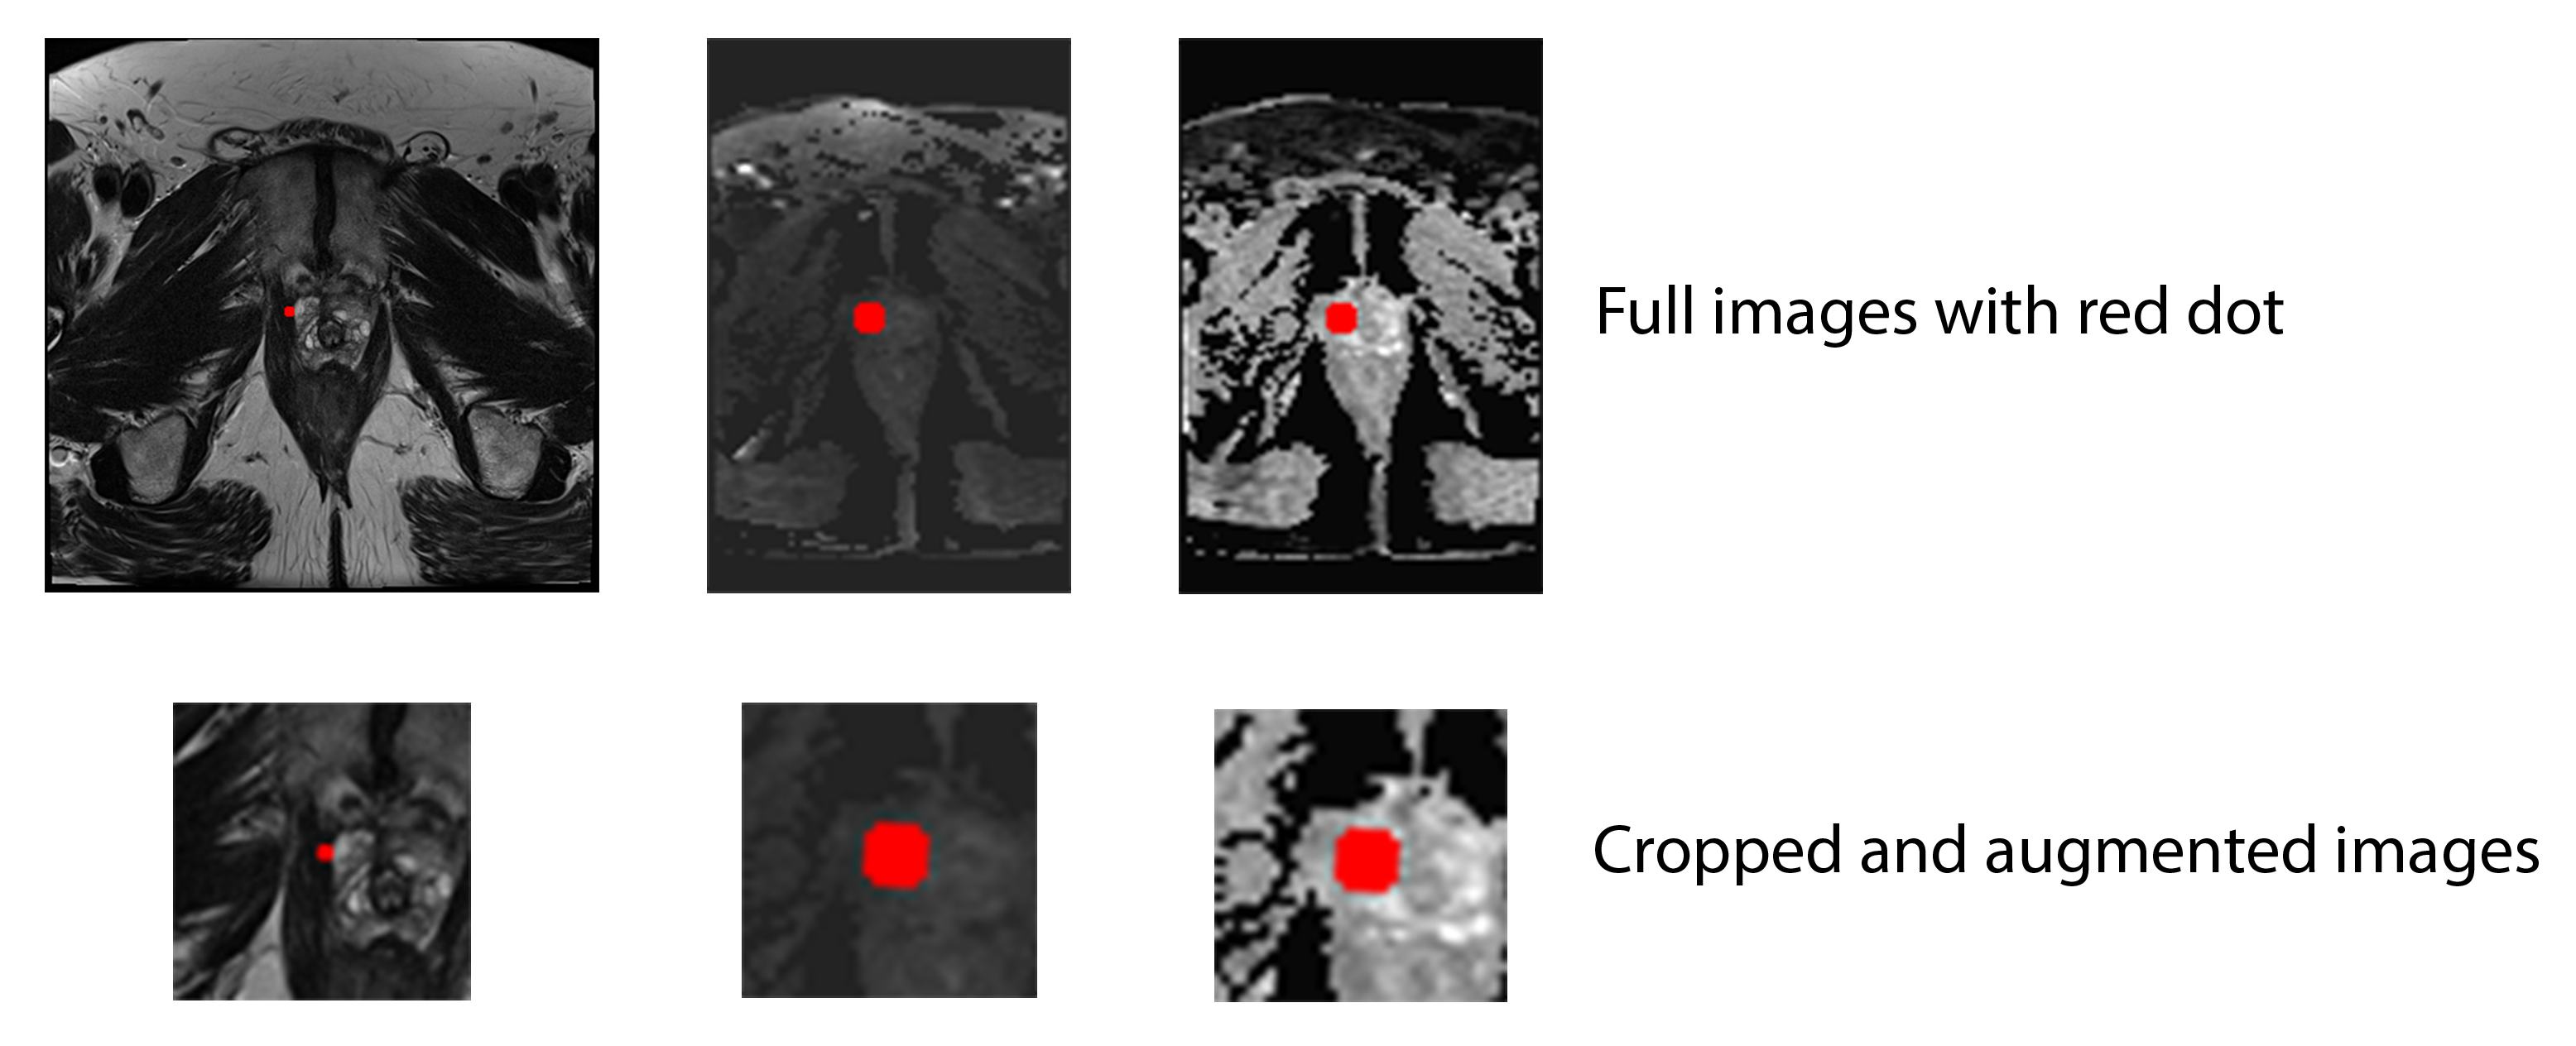
\includegraphics[width=\textwidth, keepaspectratio=true]{./figures/test_red_dot.png}
\caption{Red dot test - Patient 0082, Finding ID 1\\From left to right: T2, DWI, ADC.}
\label{fig:reddot}
\end{figure}


\subsubsection{Alignment}
In addition to the previous test, another one aiming at checking the alignment of the images was implemented. This test ensures that the three images show the exact same content at the same spot over the three channels (see Figure \ref{fig:alignment}). 

\begin{figure}[!h]
\centering
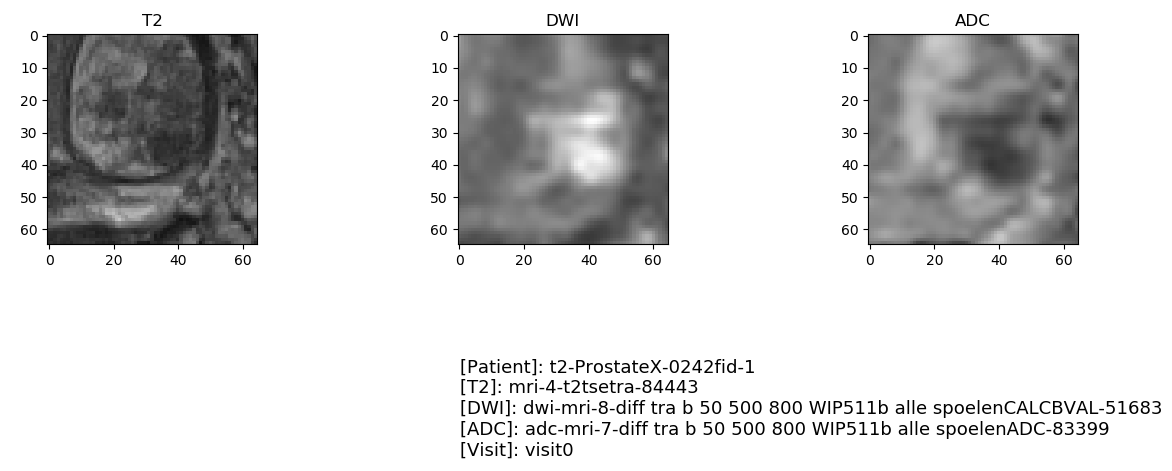
\includegraphics[width=\textwidth, keepaspectratio=true]{./figures/alignment.png}
\caption{Alignment - Patient 0242 - Finding ID 1}
\label{fig:alignment}
\end{figure}

\subsection{Training the neural network}

\setlength{\marginparwidth}{3cm}\leavevmode \marginnote{\textbf{Jobin}}Training the neural network is the most important step of the experiment after the data processing. This section first describes the architecture of the model, then presents the script used for the training and finally provides details about the experimental setup such as the training procedure, the hyperparameters of the model and the configuration of the machine on which it was trained.

\subsubsection{Architecture}
\setlength{\marginparwidth}{3cm}\leavevmode \marginnote{\textbf{Jobin}}The model architecture used in the paper is a modified version of the VGG network from the Oxford's Visual Geometry Group (VGG). This model was initially designed as part of the Large Scale Visual Recognition Challenge 2014 that used the ImageNet dataset composed of 14 million images belonging to 1000 classes. Figure \ref{fig:paper_model} illustrates its structure and its corresponding implementation in Python with the PyTorch framework.

It is first composed of three convolution-dropout-max-pooling blocks followed by three fully-connected-dropout blocks. Each convolutional box (in blue) in the figure represents in reality three layers: the convolutional layer, the batch normalization layer and the exponential linear unit (ELU) activation function. The same principle applies to the fully connected layer box (in orange) that is divided into a fully connected layer followed by the exponential linear unit. The last fully connected box (in purple) has the same structure except that the exponential linear unit is replaced with a softmax function for classification.

In comparison to the original VGG, this model keeps the small filter size of 3x3, also doubles the number of filters after each convolution-dropout-max-pooling block and has a stride of 1 for all convolutions. It differs from the traditional VGG in that it makes use of a smaller number of layers since the task is simpler than the original one. Moreover, it uses exponential linear units instead of rectified linear units as activation functions and adds dropout and batch normalization layers. Also, it uses 1x1 convolutions. 

\begin{figure}[!h]
\centering
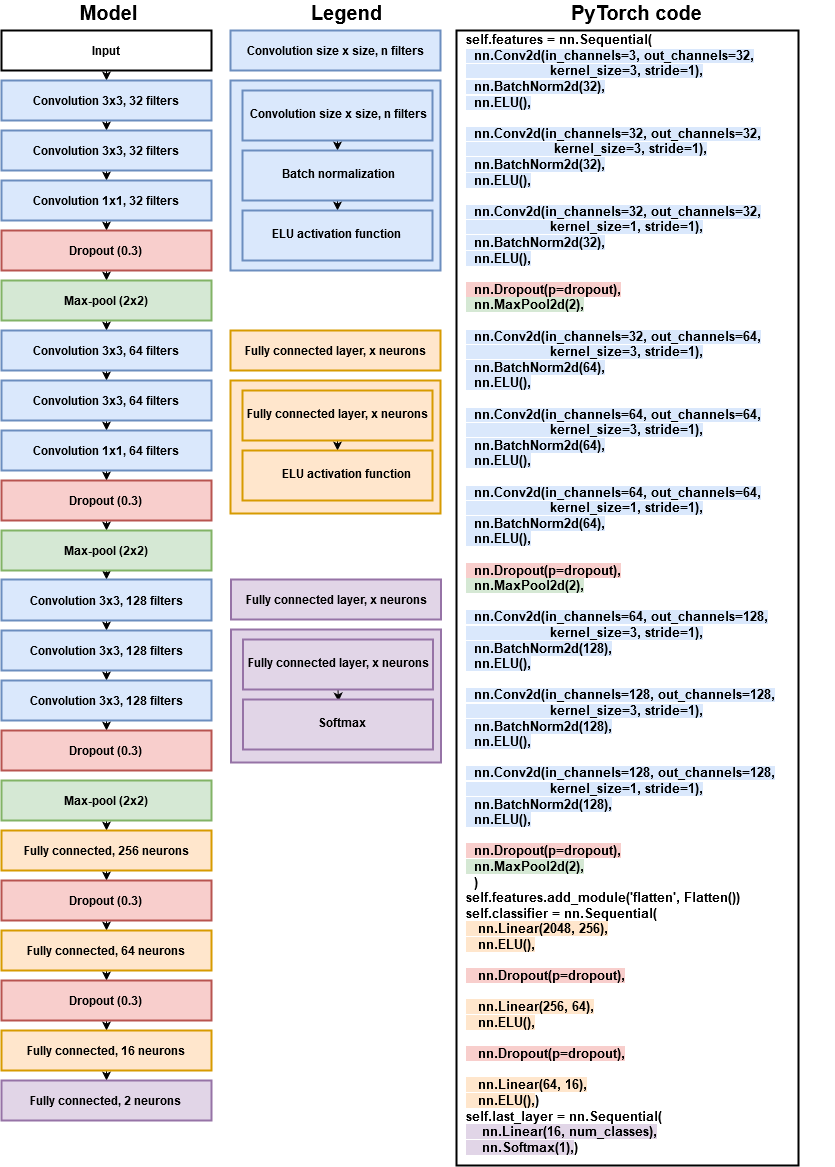
\includegraphics[width=1\textwidth, keepaspectratio=true]{./figures/model_paper_manual.png}
\caption{Model architecture with the corresponding PyTorch code}
\label{fig:paper_model}
\end{figure}

\subsubsection{Script options}
\setlength{\marginparwidth}{3cm}\leavevmode \marginnote{\textbf{Jobin}}Since training a neural network requires datasets, hyperparameters and many more configuration choices, the creation of a generic script that accepts multiple options is necessary. This requirement was solved thanks to the Python module called "argparse". The latter automatically generates help/usage messages and displays errors when the arguments typed in by the user are invalid. Table \ref{fig:paper_reproduction_options} shows all options accepted by the script, provides information about what they concretely mean and indicates their respective types.


% Please add the following required packages to your document preamble:
% \usepackage{graphicx}
% \usepackage[table,xcdraw]{xcolor}
% If you use beamer only pass "xcolor=table" option, i.e. \documentclass[xcolor=table]{beamer}
\begin{table}[!h]
\resizebox{\textwidth}{!}{%
\begin{tabular}{|llll|}
\hline
\rowcolor[HTML]{DAE8FC} 
\textbf{Command}            & \textbf{Description}                                                                                                                                                                                                & \textbf{Required}                                                           & \textbf{Type} \\ \hline
\textbf{-{}-trainingset}     & Training set  path                                                                                                                                                                                                  & True                                                                        & String        \\ \hline
\textbf{-{}-validationset}   & Validation set path                                                                                                                                                                                                 & True                                                                        & String        \\ \hline
\textbf{-{}-batchsize}        & Number of samples per batch                                                                                                                                                                                         & True                                                                        & Int           \\ \hline
\textbf{-{}-nbepochs}         & Number of epochs the training phase has to last                                                                                                                                                                     & True                                                                        & Int           \\ \hline
\textbf{-{}-lr}               & Learning rate used by the optimizer                                                                                                                                                                                 & \begin{tabular}[c]{@{}l@{}}False\\ Default: 1e-3\end{tabular}               & Float         \\ \hline
\textbf{-{}-lossfunction}     & \begin{tabular}[c]{@{}l@{}}Loss function name\\{[}CrossEntropyLoss, L1Loss, MSELoss{]}\end{tabular}                                                                                                            & \begin{tabular}[c]{@{}l@{}}False\\ Default: 'CrossEntropyLoss'\end{tabular} & String        \\ \hline
\textbf{-{}-cudadevice}      & GPU name to run the experiment                                                                                                                                                                                      & \begin{tabular}[c]{@{}l@{}}False\\ Default: 'cuda'\end{tabular}             & String        \\ \hline
\textbf{-{}-modeltoload}      & \begin{tabular}[c]{@{}l@{}}Pretrained model name \\If given, load it, otherwise randomly initialize it\end{tabular}                                                                                     & \begin{tabular}[c]{@{}l@{}}False\\ Default: ''\end{tabular}                 & String        \\ \hline
\textbf{-{}-dropout}          & Dropout probability                                                                                                                                                                                                 & \begin{tabular}[c]{@{}l@{}}False\\ Default: 0.3\end{tabular}                & Float         \\ \hline

\textbf{-{}-inputchannel}     & \begin{tabular}[c]{@{}l@{}}Number of channels of the input images\\{[}1,3{]}\end{tabular}                                                                                                            & \begin{tabular}[c]{@{}l@{}}True\end{tabular} & Int        \\ \hline

\textbf{-{}-optimizedmetric} & \begin{tabular}[c]{@{}l@{}}Metric to optimize\\ The best model during the training will be saved according to it\\{[}'auc', 'accuracy', 'precision', 'recall', 'f1score', 'specificity'{]}\end{tabular} & \begin{tabular}[c]{@{}l@{}}False\\ Default: 'auc'\end{tabular}              & String        \\ \hline
\textbf{-{}-outputdirectory}  & Root of the output directory used by Tensorboard to save the models                                                                                                                                                 & True                                                                        & String        \\ \hline
\end{tabular}%
}
\caption{Complete list of script options}
\label{fig:paper_reproduction_options}
\end{table}


\subsubsection{Tensorboard}
\setlength{\marginparwidth}{3cm}\leavevmode \marginnote{\textbf{Jobin}}Tensorboard's official website~\cite{39} claims that "Tensorboard provides the visualization and tooling needed for machine learning experimentation:
\begin{itemize}
\item Tracking and visualizing metrics.
\item Visualizing the model graph (ops and layers).
\item Viewing histograms of weights, biases, or other tensors as they change over time.
\item Projecting embeddings to a lower dimensional space.
\item Displaying images, text, and audio data"~\cite{39}.
\end{itemize}
In this experiment, Tensorboard is mainly used to plot Matplotlib figures of the model performance. In fact, during the training the following metrics are computed: loss, accuracy, precision, recall, F1-score, specificity and AUC. These metrics are computed separately on the training and on the validation sets at the end of each epoch. They are then stored and plotted on the same figure at the end of the process thanks to Tensorboard. In addition to this, written reports regarding which model was the best and the results it achieved are also added to the dashboard.
\label{paper_tensorboard}


\subsubsection{Model roulette}
\setlength{\marginparwidth}{3cm}\leavevmode \marginnote{\textbf{Cl{\'e}ment}}As stated by the authors, "the training process is sensitive to the parameter initialization" \cite{07}. Experience showed us that the exact same hyperparameters with two different initializations could give opposite results. Therefore, in order not to train the model vainly, a script which generates a given number of initializations was created. Each untrained model was then tested on the validation set since the best model during training is saved according to its performance on the validation set. The model whose score was the highest on a given metric (the AUC in this experiment) was saved and used as base model for the experiments. It can then be used as initialization model using the script option \textit{-{}-modeltoload <path>}.



\subsubsection{Experimental setup}

\setlength{\marginparwidth}{3cm}\leavevmode \marginnote{\textbf{Jobin}}Keeping the exact same hyperparameters as the original paper led the experiment to disappointing results. Consequently, new hyperparameters had to be found. A grid search approach driven by the AUC obtained on the test set (the one built for the experiment, not the one of the challenge) was chosen. In practical terms, this consisted in trying multiple combinations of hyperparameters and keeping the one that produced the best AUC on this test set. At the end of this process, it appeared that the best model was obtained when the data was organized in batches of 32 samples, with an initial learning rate of $1*10^{-7}$, a learning rate scheduler on plateau using a factor of 100 with a patience of 2 (the learning rate is divided by 100 when the validation AUC decreases for two consecutive epochs) and a dropout rate of 0.2. Note that the model was initialized picking the best one among 200 models generated from a roulette maximizing the AUC. This model was implemented with PyTorch using the Adam optimizer to update its weights and was trained on an Nvidia GeForce GTX Titan X graphics card during approximately 3 hours.\\

\subsection{Training verification}
\setlength{\marginparwidth}{3cm}\leavevmode \marginnote{\textbf{Jobin}}In deep learning, two main problems can occur during training. The first one is called the "vanishing gradient" problem and refers to the fact that it is possible for the loss function to compute extremely small gradients, near zero. Consequently, the weight update is also extremely small, which makes the neural network hard or impossible to train. The second problem, the "exploding gradient" is the opposite. In this case, large gradients are computed, which leads to huge weight updates that can even reach "NaN" values. This makes the model unstable and unable to learn from training data.

As a result, it is important to analyse the gradient propagation across the network to ensure that it is not facing such problems. To achieve this goal, a visualization tool to display the gradients of the entire network was implemented. This implementation is based on the code of RoshanRane~\cite{47}.  This allows to visually notice the gradient flow at a glance and to see its evolution throughout all epochs (one visualization per batch is generated).


\subsubsection{Gradient flow visualization}
The visualization displays the gradient flow through the entire neural network. It shows the name of each layer on the x-axis and its average gradient value on the y-axis (recall: for each layer the gradient is a matrix). Furthermore, it also gives information about the max value of the gradient and indicates in black if one of them is equal to zero.

Figure \ref{fig:gradient_flow} shows the gradient flow at epoch 0, batch 6. From the output layer (called "last\_layer0.weight" on the graph) to the first layer, the gradient is well propagated: no huge average gradients are registered, neither extremely small ones. The training process goes on correctly.

\begin{figure}[!h]
\centering
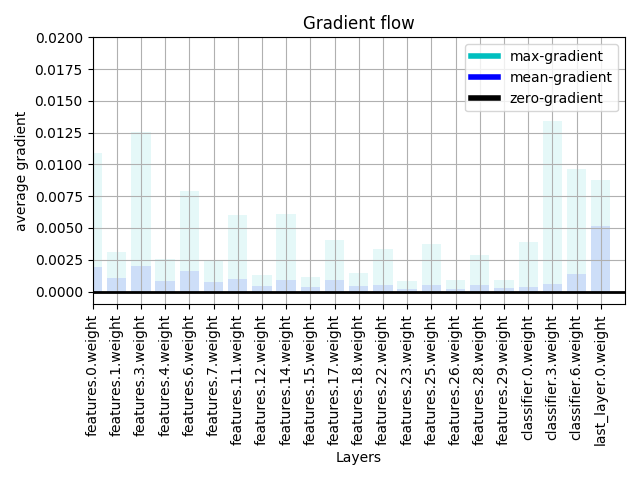
\includegraphics[width=1\textwidth, keepaspectratio=true]{./figures/gradient_flow.png}
\caption{Gradient flow at epoch 0 of the experiment, batch 6}
\label{fig:gradient_flow}
\end{figure}


\subsection{Results}
\label{sec:paper_reproduction_results}
\setlength{\marginparwidth}{3cm}\leavevmode \marginnote{\textbf{Jobin}}Figure \ref{fig:paper_reproduction_results} shows the different metrics registered on the training and validation sets during the training phase. The best model was chosen at epoch 21 with an accuracy of $0.7525$ and an AUC of $0.765$ on the validation set (recall: the condition for a model to be chosen as best is that the current AUC and accuracy should be higher than the AUC and accuracy of the previous best model).

\noindent This best model was evaluated on the test set built for the experiment and achieved an AUC of $0.75$ using their "enhanced prediction" technique (see Figure \ref{fig:paper_reproduction_auc_on_our_test_set}).

Finally, the model was also tested on the official SPIE-AAPM-NCI Prostate MR Classification Challenge test set and achieved an AUC of 0.71 (see Figure \ref{fig:paper_reproduction_results_challenge_1}). This result will be used as a benchmark in comparison with the model trained on the whole dataset in the second part of the experiment.

\newpage

\begin{figure}[!h]
\centering
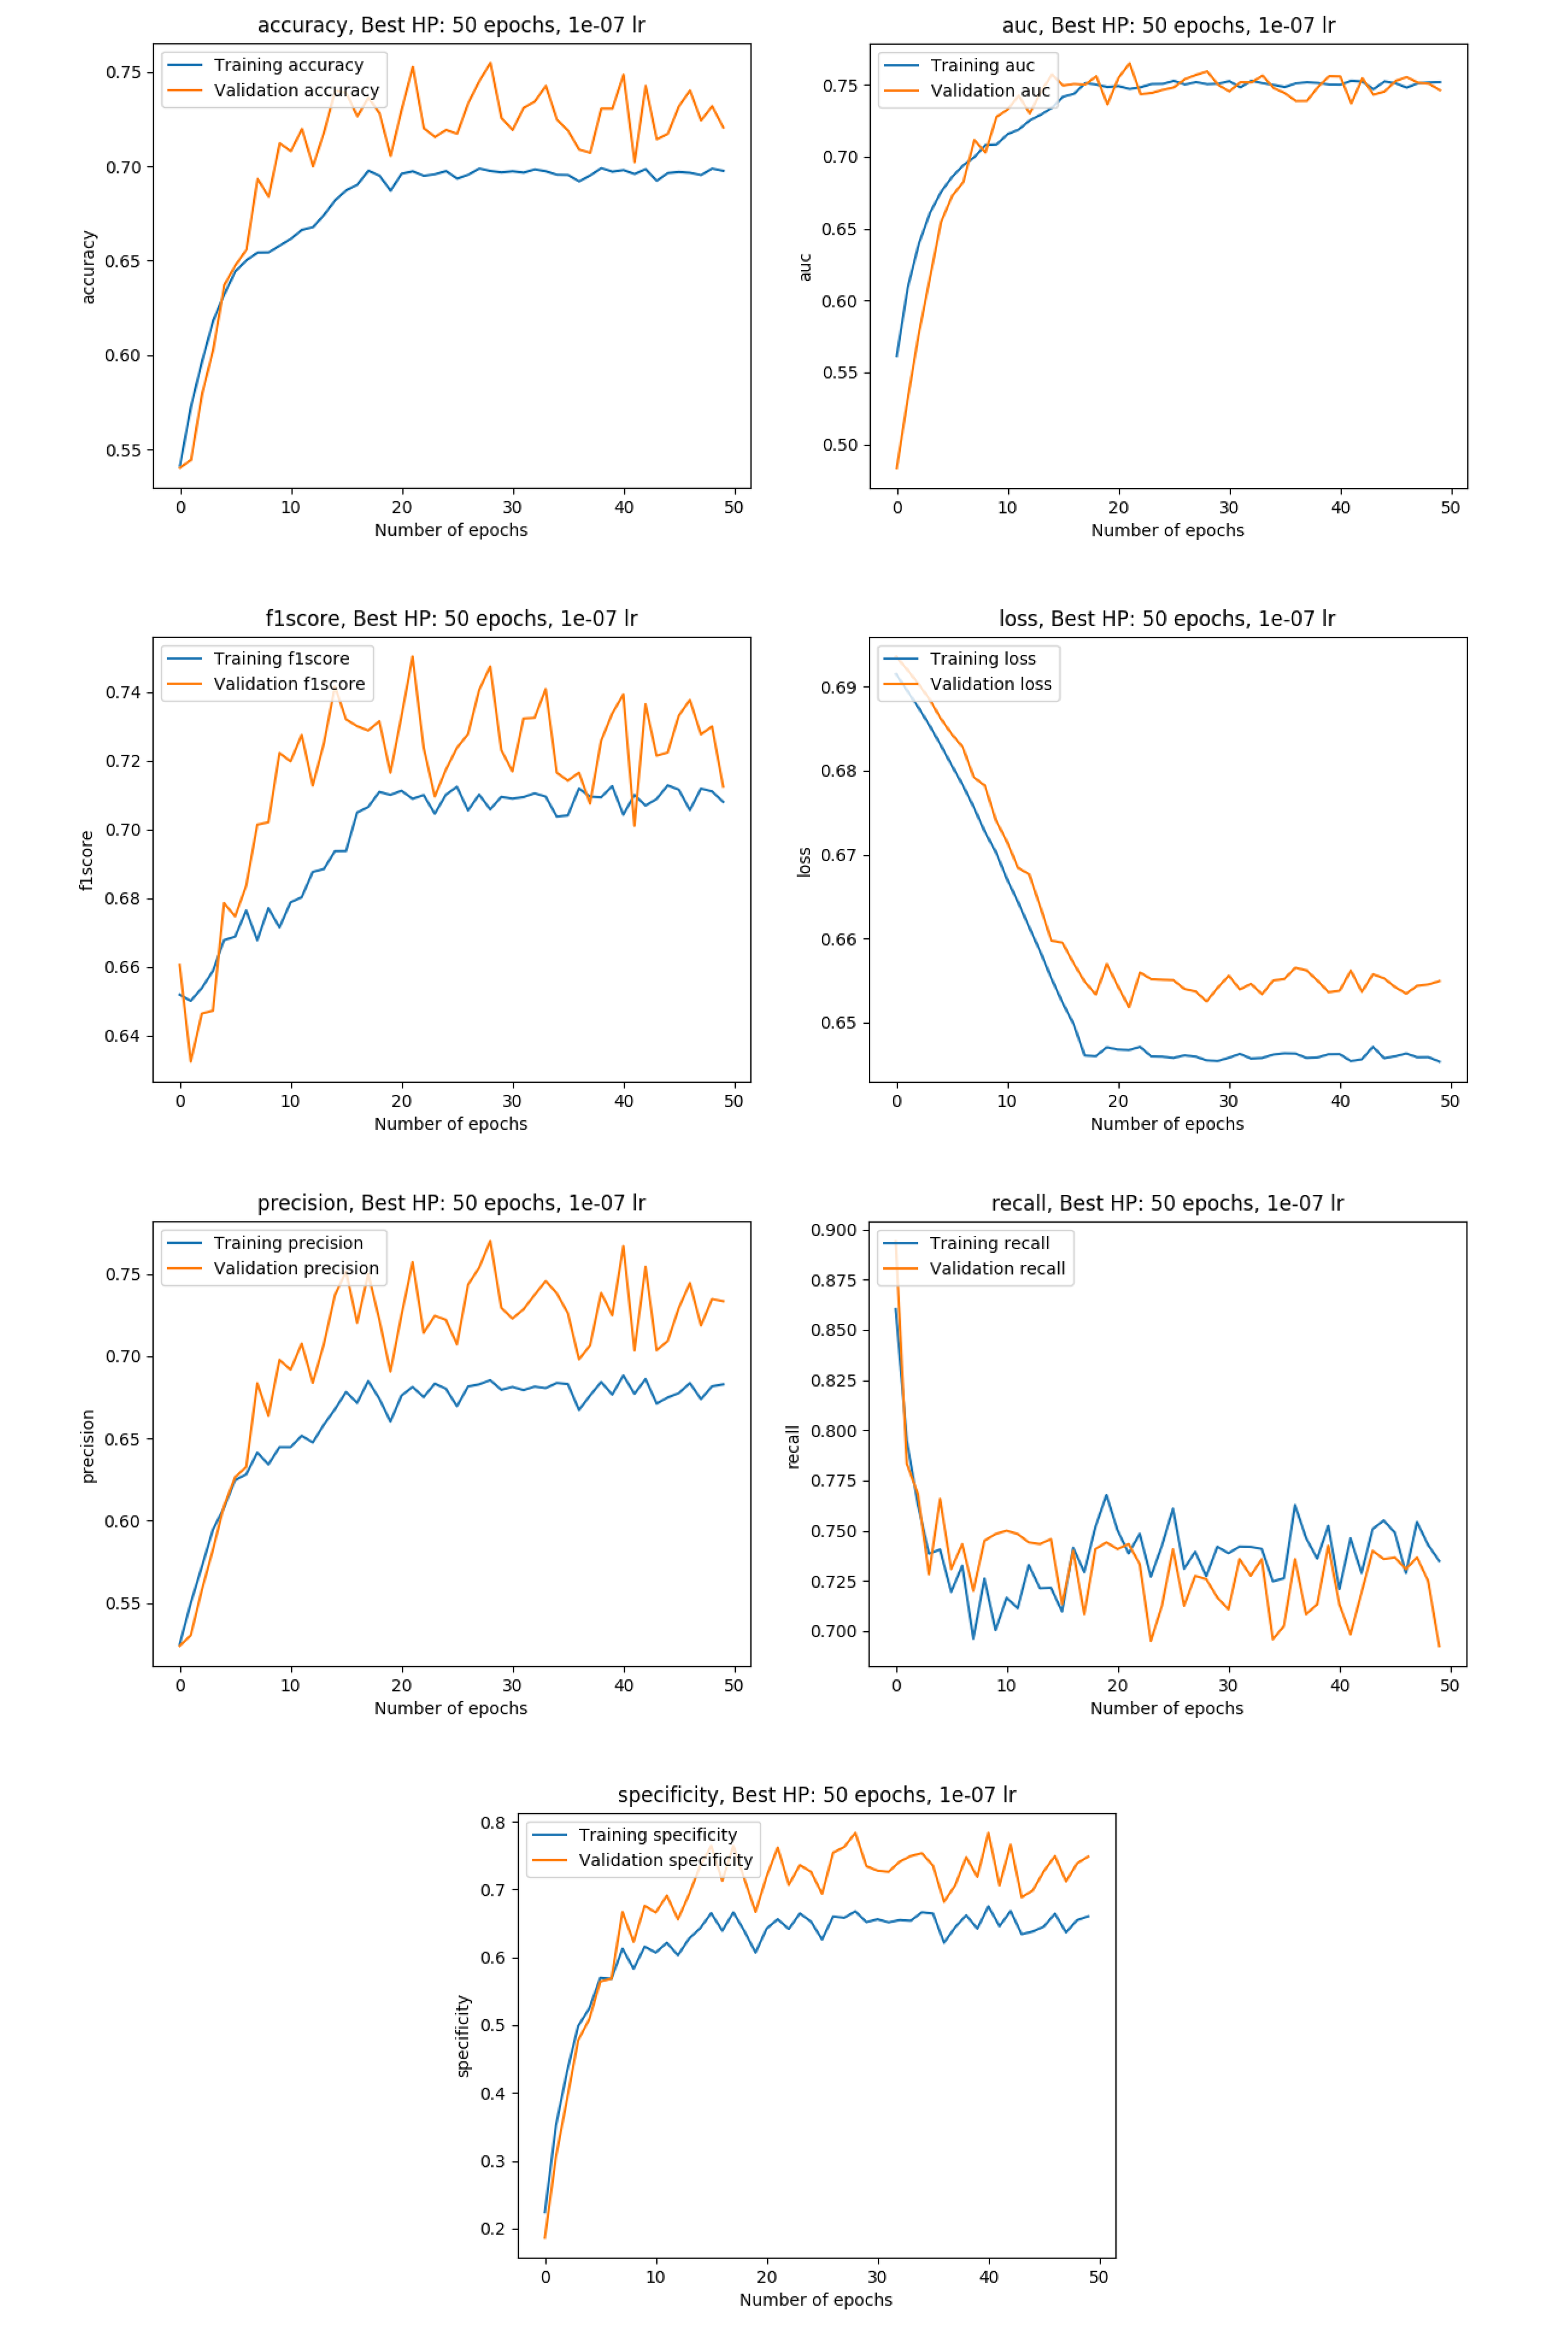
\includegraphics[width=1\textwidth, keepaspectratio=true]{./figures/paper_reproduction_results.png}
\caption{Metrics on the training and validation sets}
\label{fig:paper_reproduction_results}
\end{figure}



\begin{figure}[!t]
\centering
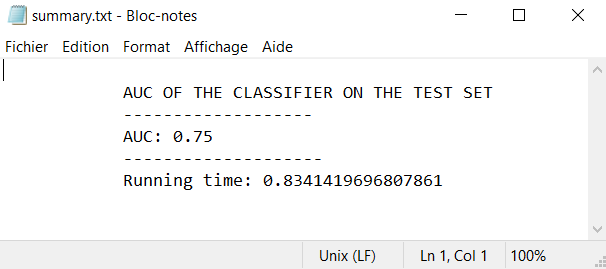
\includegraphics[width=0.6\textwidth, keepaspectratio=true]{./figures/auc_our_test_set.png}
\caption{AUC of the best model on our test set}
\label{fig:paper_reproduction_auc_on_our_test_set}
\end{figure}

\begin{figure}[!t]
\centering
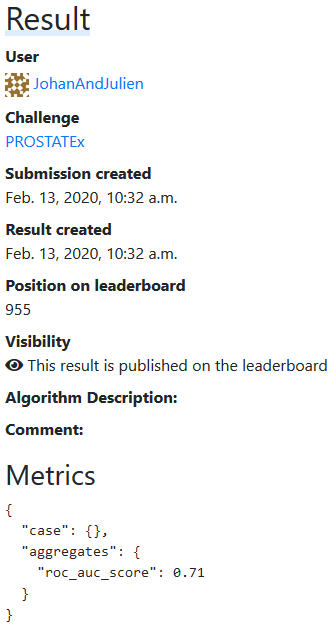
\includegraphics[width=0.6\textwidth, keepaspectratio=true]{./figures/paper_reproduction_results_challenge1.png}
\caption{Score achieved on the PROSTATEx challenge only using our custom training set (80\% of all available data) for the training}
\label{fig:paper_reproduction_results_challenge_1}
\end{figure}


\subsection{Discussion}
\setlength{\marginparwidth}{3cm}\leavevmode \marginnote{\textbf{Jobin}}Thanks to the curves of Section \ref{sec:paper_reproduction_results}, a lot of information regarding the model performance can be inferred. In fact, as stated by Jason Brownlee, "reviewing learning curves of models during training can be used to diagnose problems with learning, such as an underfit or overfit model, as well as whether the training and validation datasets are suitably representative"~\cite{40}.

First of all, when observing the loss plot, it is noticeable that the training and validation losses have the same behavior during the 50 epochs. This is a clear sign of good fit of the model on the data. All the features learned by the model on the training data are also applicable to the validation set. This situation is the optimal one. Regarding the slope of the curve, a big change occurs at epoch 17. This moment corresponds to the one where the learning rate is reduced by a factor of $100$ thanks to the \textit{reducelronplateau} function. In fact, at this moment, the validation AUC (the training is optimized according to this metric) is at its optimum with this learning rate. If this technique had not been used, the training loss would have continued to go down whereas the validation loss would have gone up immediately, which would have led to overfitting. Here, thanks to the learning rate scheduler, this scenario is avoided as the validation and training losses stay stable from this point onwards. The same behaviour is clearly noticeable for all other metrics.

Regarding the overall performance of the best model chosen at epoch 21, the latter generalizes well. This is particularly visible on the accuracy and AUC plots where the validation metrics are higher or equal to the training ones. The validation accuracy indicates that the model makes the right class decision in approximately $75$\% of the time. Furthermore, as the model achieves a validation AUC of $0.76$, it shows that it has a good distinction capacity. In fact, the highest the AUC is, the highest is the ability of the model to predict benign lesions as benign and malignant lesions as malignant. Armato et al.~\cite{42} claim that a less-experienced radiologist can reach an AUC of $0.81$ and an expert an AUC of $0.91$. Consequently, this model is almost at the level of a radiologist, which is very promising. It is also important to keep in mind that the model was trained using only 164 patients (80\% of the 204 training patients), which suggests that even better results can be reached with more data.

The precision plot, which is used to measure the proportion of malignant lesions correctly classified among all lesions classified as malignant lesions, confirms the hypothesis that the model has a good distinction capacity with a score of approximately $0.76$ on the validation set.

\noindent Another extremely important aspect in the medical field is to avoid the number of false negatives as much as possible. In fact, the consequences of classifying a malignant lesion as benign are far worse than the opposite. This concept is measured by the recall, which quantifies the proportion of malignant lesions correctly classified among all malignant lesion. The model has a recall of around $0.74$ on the validation set.

\noindent The two last metrics (precision and recall) are both considered in the f1-score that is equal to $0.76$.

\noindent Finally, the specificity indicates the proportion of correctly classified benign lesions among all benign lesions and is equal to approximately $0.76$.

\noindent Globally, this model is balanced as no metric is exploding at the expense of another. This stability constitutes a serious strength regarding its generalization ability.

As the goal of the experiment was to reproduce the experiment of the paper, a comparison between the two models is necessary. The reproduced model achieves an AUC of $0.75$ on our test set (see Figure \ref{fig:paper_reproduction_auc_on_our_test_set}) using the authors' "enhanced prediction" technique, whereas the authors achieved an AUC $\in [0.876-0.994]$ with 95\% of confidence on their test set. Consequently, the model presented in this work has a slightly smaller AUC of $[0.126-0.244]$ than the one achieved in the paper. Multiple factors can explain this difference. 

First, in their work, the lesion cropping was performed by a qualified radiologist, whereas, in our case, it was automatically done using the information in the CSV files. Then, the way the test set is built can make the results vary a lot. In fact, the authors did not provide any information about how they built their test set. It is therefore possible that the test set was chosen to maximize the performance of the model. In the current work, the test set is built randomly. Consequently, the comparison of the performance is difficult since the test set is not the same in the two works. The only way to seriously compare the two models would be to compare their performance on the official SPIE-AAPM-NCI Prostate MR classification challenge test set. The model of this section (trained with 80\% of all the data available) reached an AUC of $0.71$. Unfortunately, no information about the performance of the model of the paper is given. Knowing that the best result at the time of the challenge was an AUC of $0.87$ on the challenge test set, it is highly surprising not to take part in it when claiming an AUC in the interval $[0.876-0.994]$ with 95\% of confidence. Finally, another source of difference is the number of participants in the experiment and the level of experience they have. Indeed, seven authors contributed to the paper, including one student with a Bachelor degree and six PhD with one of them working for Siemens Healthcare and one for hImagingTek Ltd. These big companies are specialized in medical imaging and have departments dedicated to machine learning. On the opposite, this work was produced independently by two MSc students without previous experience in the medical imaging field. 

\newpage
\section{SPIE-AAPM-NCI Prostate MR Classification Challenge}
\label{sec:classification_challenge}
\setlength{\marginparwidth}{3cm}\leavevmode \marginnote{\textbf{Jobin}}This section aims at maximizing the result on the SPIE-AAPM-NCI Prostate MR classification Challenge test set by using the entire dataset as training set, instead of using 80\% of it, as it was done in the previous section. First, the changes needed to reach this new goal are detailed, then the raw results are presented and the latter are finally interpreted.

\subsection{Training the neural network with the whole dataset}
\setlength{\marginparwidth}{3cm}\leavevmode \marginnote{\textbf{Jobin}}The first part of the experiment, in which the whole dataset was split into a training (80\%), a validation (10\%) and a test set (10\%), was extremely useful to find the right hyperparameters. It also gave the opportunity to check that the model and the processing of the data worked as expected with the goal of creating a state-of-the-art deep learning model for prostate lesion classification.

As a complement, this part of the experiment focuses on the challenge results in order to improve the AUC of $0.71$ achieved by the model trained with 80\% of all available data. In a general way, the more available data there is, the better the model performs. Consequently, the idea behind this section is to use the entire dataset as training set, discarding the validation and test sets from previous section. Apart from this new split, the data processing and the hyperparameters stay the same. The only difference in the training is about the learning rate scheduler. Since the validation set does not exist anymore, there is no possibility to use the \textit{reducelronplateau} function to prevent overfitting. However, this does not cause any problem thanks to the results of the previous section. In fact, it is clearly visible that the model would have started overfitting at epoch 17 if no learning rate correction had been applied. Hence, it is possible to conclude that, in this case, the best model should also be the one around epoch 17 (or a few epochs later). In order to ensure this, the models at epochs 15, 16, 17, 18, 19, 20, 21, 22, 23 and 30 were evaluated on the official challenge test set. For each of these models, a CSV file containing the predictions for each lesion of each patient was automatically generated and submitted to the challenge.

\subsection{Results on the challenge test set}
\setlength{\marginparwidth}{1.5cm}\leavevmode \marginnote{\textbf{Jobin}}Figure \ref{fig:challenge_all_results_experiment} presents the metric values the model reached while training on the whole dataset. The models whose results are reported in Table \ref{fig:results_for_all_models_challenge} were picked from this training.

\noindent Table \ref{fig:results_for_all_models_challenge} shows the AUC values achieved by the model on the official challenge test set. The range of values is contained in the interval $[0.75-0.76]$. Each model was tested in order to see if a slight peak of $0.01$ could be found from one epoch to the other.

\noindent Finally, Figure \ref{fig:paper_reprodution_results_challenge2} shows our participation to the challenge with the model picked at epoch 20, which achieved an AUC of $0.76$.

\newpage

\begin{figure}[!h]
\centering
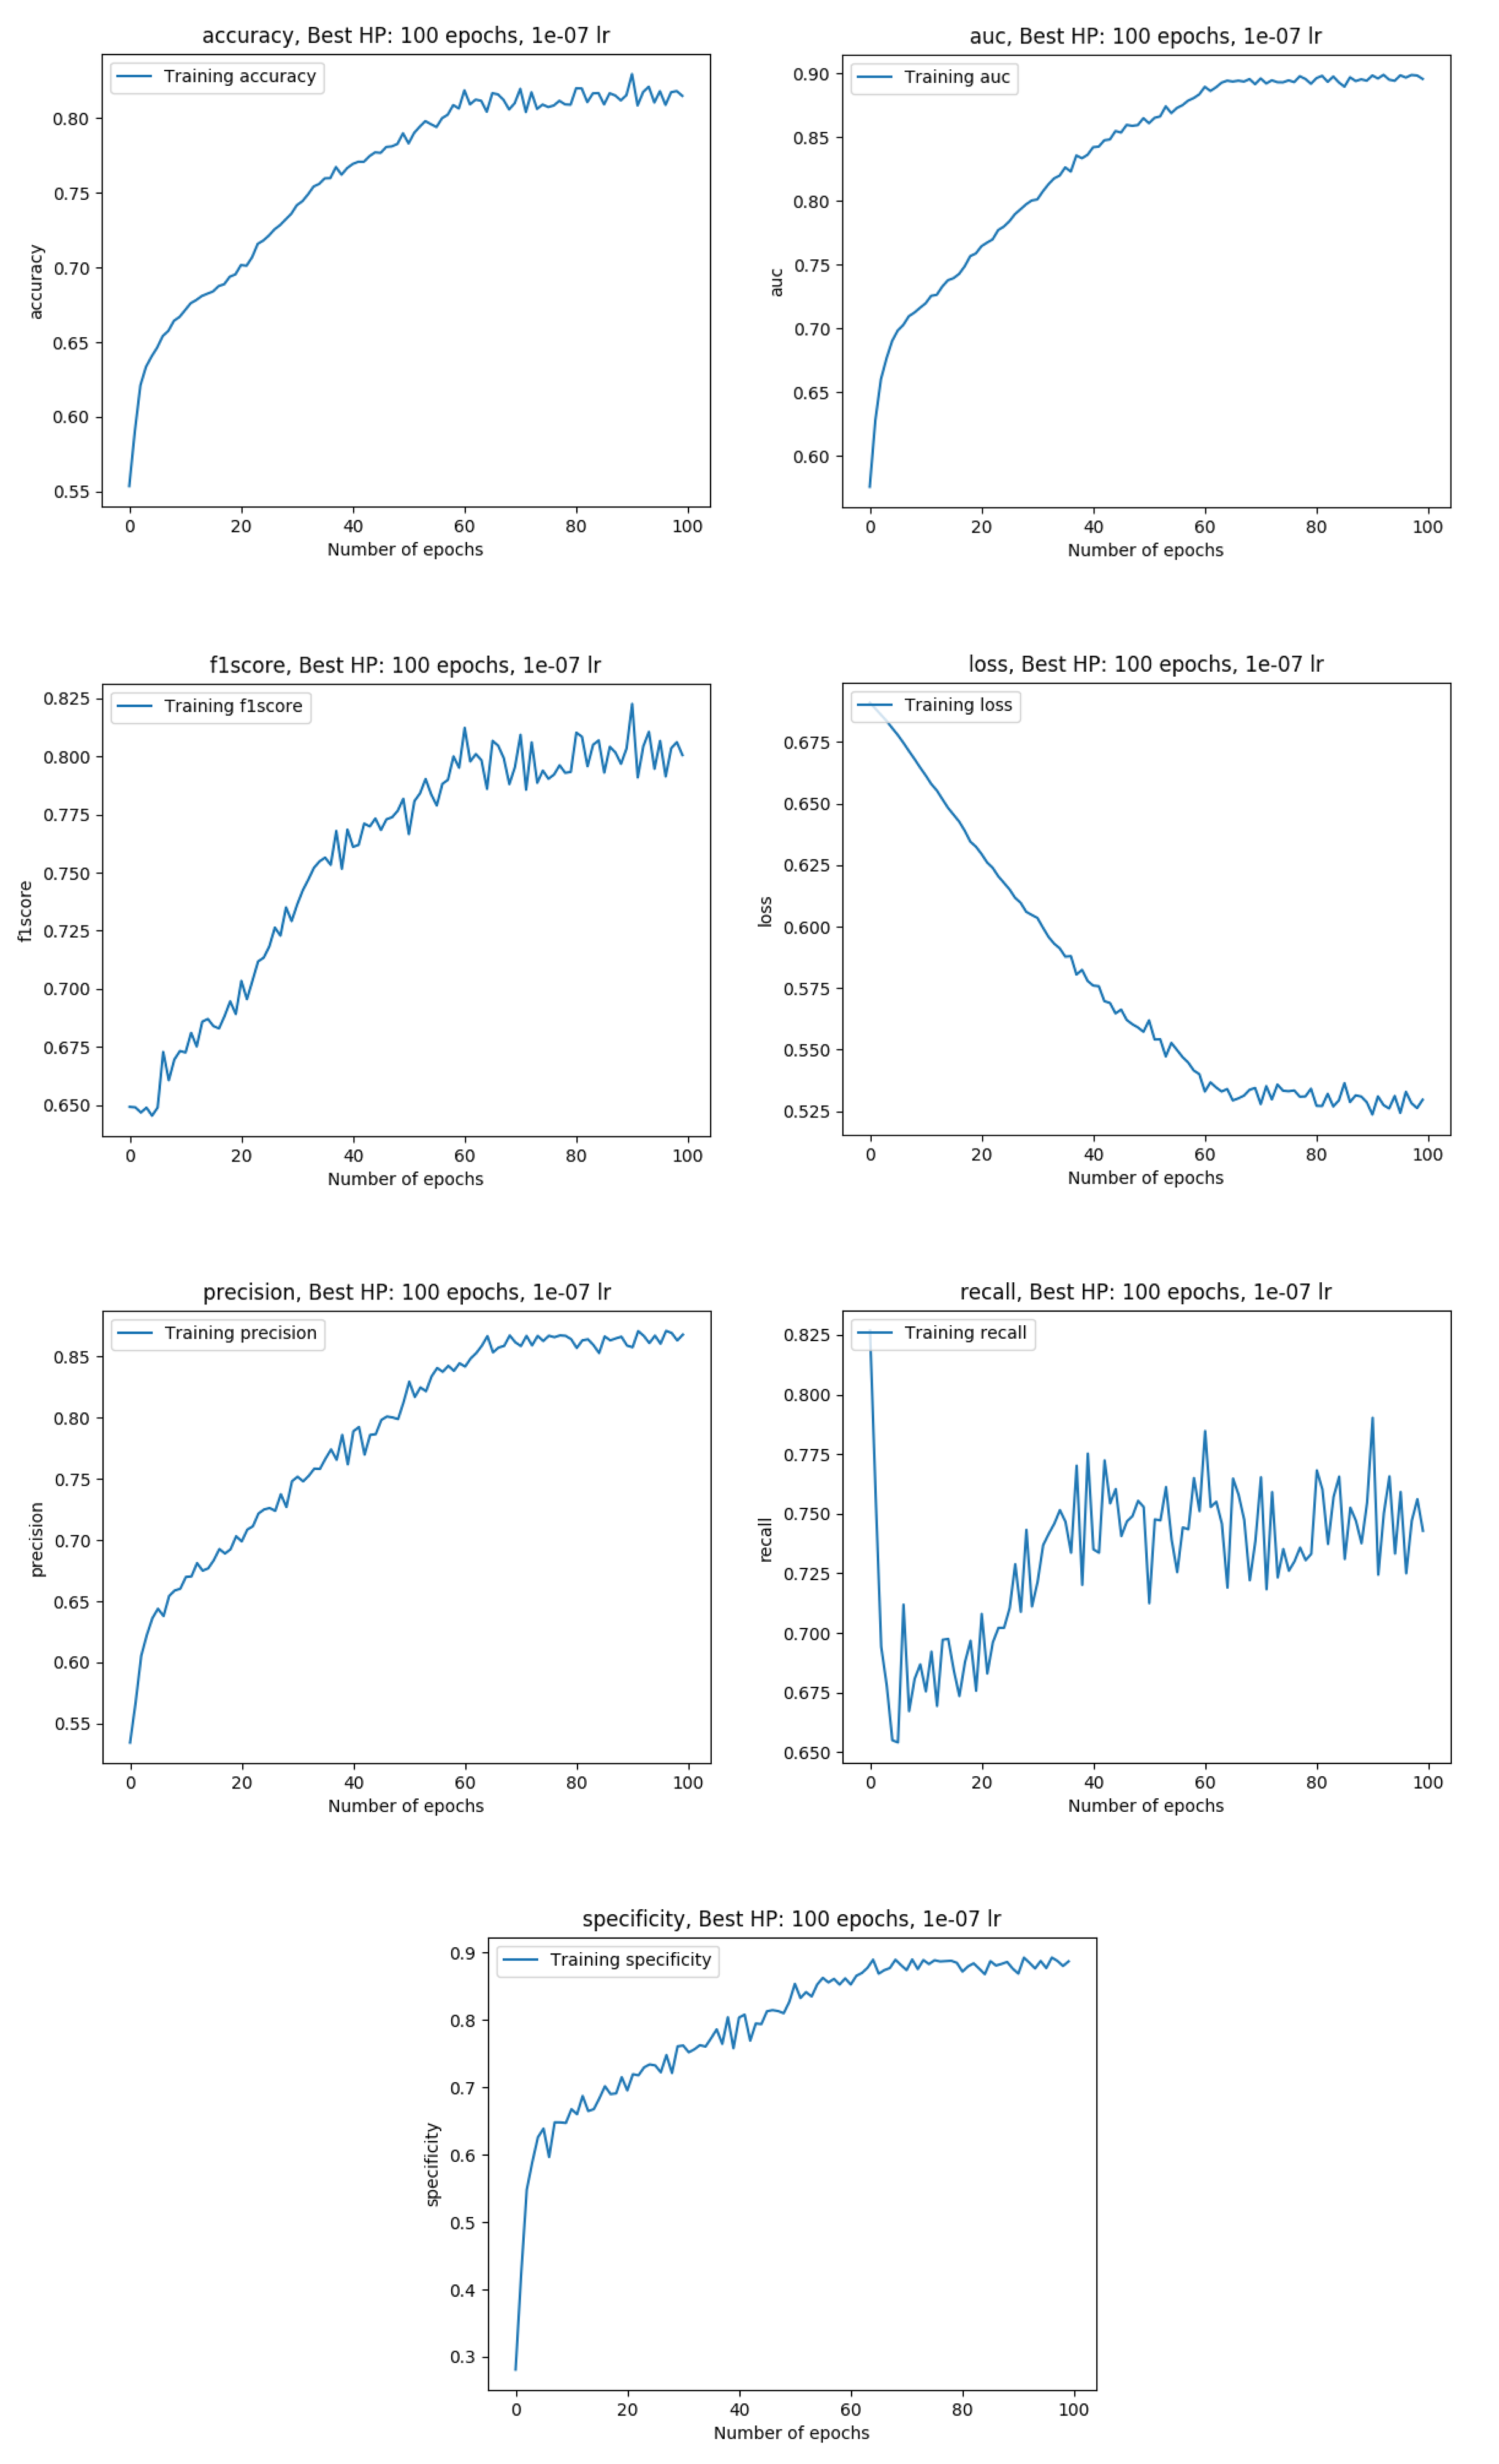
\includegraphics[width=0.95\textwidth, keepaspectratio=true]{./figures/paper_reproduction_results_challenge_full_dataset.png}
\caption{Metrics on the training using all data available as training set}
\label{fig:challenge_all_results_experiment}
\end{figure}

\begin{table}[!t]
\resizebox{\textwidth}{!}{%
\begin{tabular}{|l|l|l|l|l|l|l|l|l|l|l|}
\hline
\rowcolor[HTML]{DAE8FC} 
\textbf{Epoch} & \textbf{15} & \textbf{16} & \textbf{17} & \textbf{18} & \textbf{19} & \textbf{20} & \textbf{21} & \textbf{22} & \textbf{23} & \textbf{30} \\ \hline
AUC            & 0.75        & 0.75        & 0.76        & 0.76        & 0.76        & 0.76        & 0.76        & 0.76        & 0.75        & 0.75        \\ \hline
\end{tabular}%
}
\caption{AUC of the model saved at different epochs on the official SPIE-AAPM-NCI Prostate MR classification test set }
\label{fig:results_for_all_models_challenge}
\end{table}

\begin{figure}[!t]
\centering
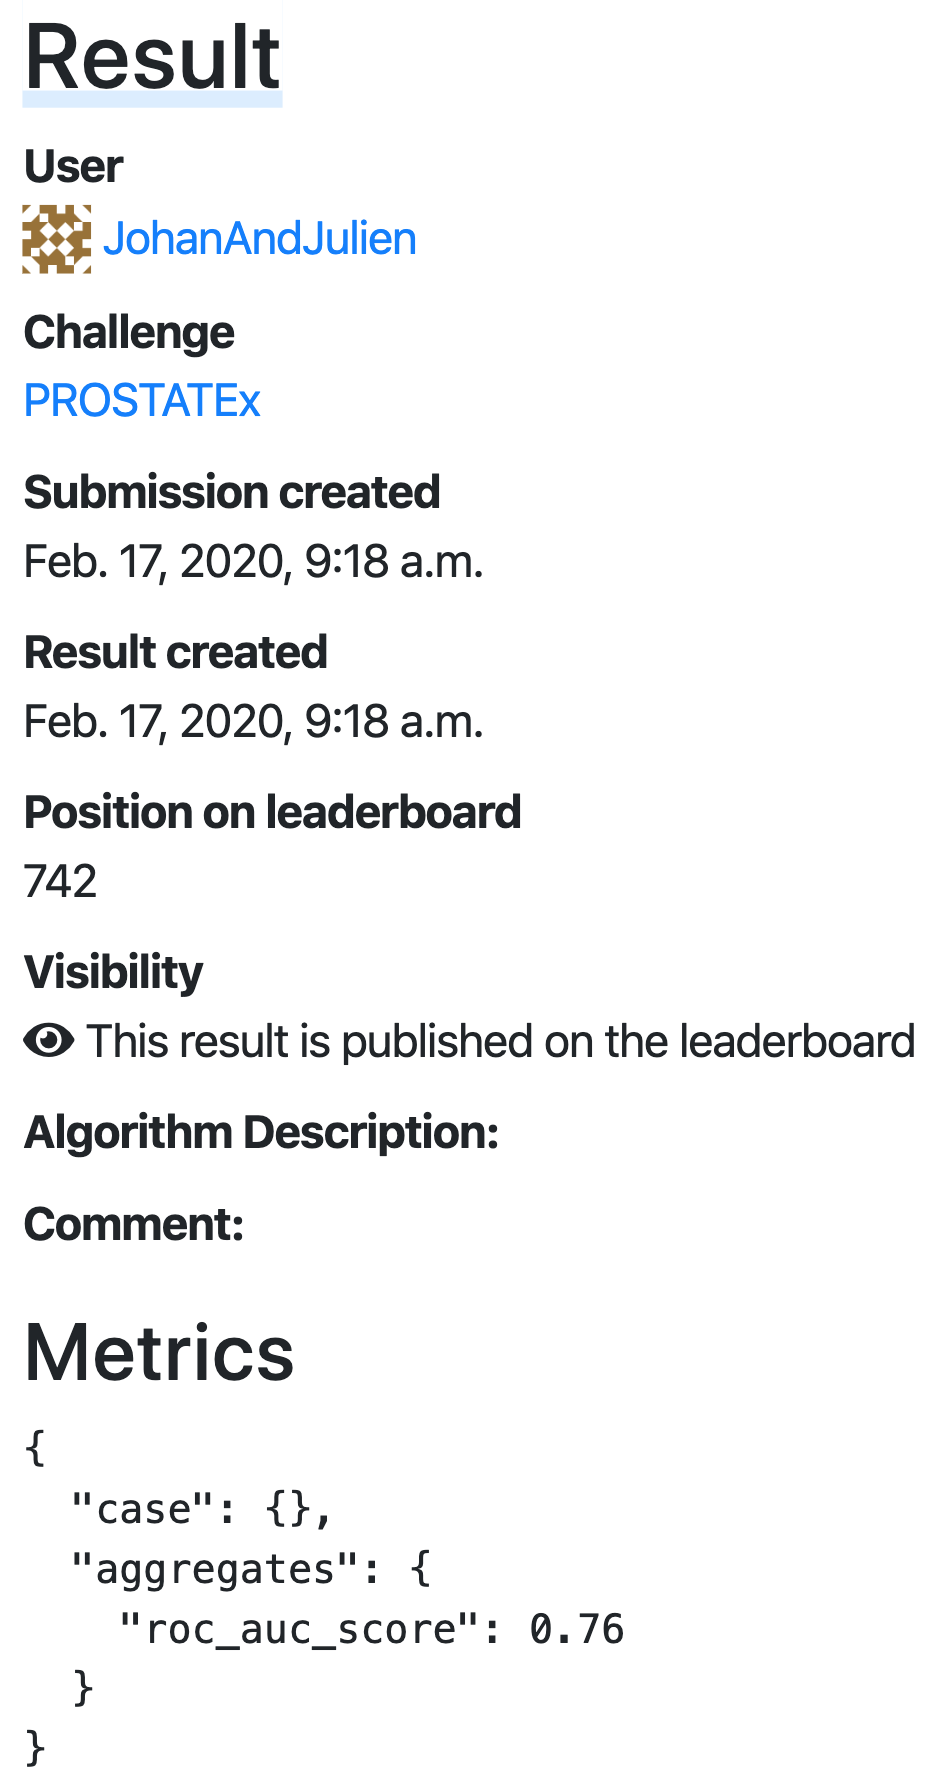
\includegraphics[height=1\textwidth, keepaspectratio=true]{./figures/paper_reproduction_results_challenge2.png}
\caption{Score achieved in the PROSTATEx challenge by the model picked at epoch 20, trained on all available data as training set}
\label{fig:paper_reprodution_results_challenge2}
\end{figure}

\clearpage

\subsection{Discussion}
\setlength{\marginparwidth}{3cm}\leavevmode \marginnote{\textbf{Jobin}}Figure \ref{fig:challenge_all_results_experiment} illustrates once again the correct behavior of the model during the training. All metrics reach their point of convergence at some point, the curves do not oscillate much and the loss curve is continually decreasing, which is a good learning indicator. In comparison to the the first part of the experiment, it is clearly visible that the metrics have a higher best value. This is due to the absence of learning rate scheduler during the training. As a result, from a certain epoch onwards, features learned by the model are not transposable to unseen data anymore and the latter overfits the data. To determine this point, multiple models around \mbox{epoch 20} were evaluated on the challenge test set (see Figure \ref{fig:results_for_all_models_challenge}). It is noticeable that the model did not reach its best performance before epoch 15 and that it started overfitting after epoch 23. Every model between these two epochs achieved an AUC of $0.76$ on the challenge, which seems to be the optimum value with this data and this configuration.

In comparison to the model of the previous section trained on 80\% of the available data, this new one improves the performance by $0.05$ (AUC of $0.76$ vs $0.71$). This is a clear indication that the more data there is, the better the model performs.

Finally, regarding the overall leaderboard of all challenge participants at the time of the challenge, the model would have been well ranked. Indeed, according to the 71 submissions to the PROSTATEx challenge (see Figure \ref{fig:challenge_all_results}), the AUC of $0.76$ achieved in this work would have placed the model at the 15$^{th}$ position overall.
